\documentclass[12pt]{report}
\usepackage[ansinew]{inputenc}
\usepackage[T1]{fontenc}
\usepackage{latexsym}
\usepackage{fixltx2e}
\usepackage[lofdepth,lotdepth]{subfig}
\usepackage{graphicx,epstopdf}
\usepackage[absolute]{textpos}
\usepackage[english]{babel}
%\usepackage[latin1]{inputenc}
\usepackage{amsmath,amsfonts}
\usepackage{natbib}
\usepackage{fancyhdr}
\usepackage{wrapfig}
\usepackage{float}
\usepackage[Conny]{fncychap}
\usepackage[usenames,dvipsnames]{color}
\usepackage{color, colortbl}
\usepackage{longtable}
\usepackage{multirow}
\usepackage{algorithmic}
\setcitestyle{numbers,open={[},close={]}}
\usepackage{epsfig}
\usepackage[official,right]{eurosym}
\usepackage{rotating}
\usepackage{hyperref}
\usepackage{rotating}
\hypersetup{pdfborder={0 0 0}}
\usepackage[absolute]{textpos}
\usepackage[rounded]{syntax}
\usepackage{appendix}
\grammarparsep 1pt
\usepackage{xyling}
\usepackage{pdfpages}

\usepackage{slashbox}
\usepackage{verbatim}
\usepackage{float}

\newfloat{Code}{H}{myc}
\allowdisplaybreaks


% Color definitions
\definecolor{light-gray}{gray}{0.95}
% Color definitions


%EPS images snask

%\usepackage{epstopdf}

\newif\ifpdf
\ifx\pdfoutput\undefined
   \pdffalse
\else
   \pdfoutput=1
   \pdftrue
\fi
\ifpdf
   \usepackage{graphicx}
   \usepackage{epstopdf}
   \DeclareGraphicsRule{.eps}{pdf}{.pdf}{`epstopdf #1}
   \pdfcompresslevel=9
\else
   \usepackage{graphicx}
\fi
%eps image snask end
\epstopdfsetup{suffix=}

%semantic udtryk
\usepackage{turnstile}
%$\nststile{Bottom}{Top}$

%\usepackage[tt]{titlepic}


%LOL MARTIN!
%End lool martin

% C# lol?
\usepackage{listings}
% default words comes from lstlang1.sty
\lstset{language=Java,
  basicstyle=\ttfamily\footnotesize\bfseries,
  float,
  columns=flexible,
  morekeywords=[1]{TmdbAPI,TmdbMovie},
  %keywordstyle=[1]\sffamily,
  backgroundcolor=\color{light-gray},
  captionpos=b,
  frame=single,
  breaklines=true, 
  keywordstyle=\color{Blue},
  commentstyle=\color{Green},
  stringstyle=\color{Mahogany},
  showspaces=false,
  showstringspaces=false,
  numbers=left,                   % where to put the line-numbers
  numberstyle=\footnotesize,      % the size of the fonts that are used for the line-numbers
  stepnumber=1
  }  \newenvironment{program}


% Code environment definition --- Java
% Usage 1: \lstinputlisting[style=sw6Java,label=something,caption=Tove]{someFile or someActualCode}   --- is shown in \listoflistings
% Usage 2: \lstinline[style=sw6Java]{someCode}   --- is not shown in \listoflistings
\lstdefinestyle{sw6Java} {
  language=Java,
  basicstyle=\ttfamily\footnotesize\bfseries,
  float,
  columns=flexible,
  morekeywords=[1]{TmdbAPI,TmdbMovie},
  %keywordstyle=[1]\sffamily,
  backgroundcolor=\color{light-gray},
  captionpos=b,
  frame=single,
  breaklines=true, 
  keywordstyle=\color{Blue},
  commentstyle=\color{Green},
  stringstyle=\color{Mahogany},
  showspaces=false,
  showstringspaces=false,
  numbers=left,                   % where to put the line-numbers
  numberstyle=\footnotesize,      % the size of the fonts that are used for the line-numbers
  stepnumber=1
}

% Code environment definition --- Java

\usepackage{url}

\definecolor{javared}{rgb}{0.6,0,0} % for strings


\definecolor{javagreen}{rgb}{0.25,0.5,0.35} % comments

\definecolor{javapurple}{rgb}{0.5,0,0.35} % keywords

\definecolor{javadocblue}{rgb}{0.25,0.35,0.75} % javadoc

 
\usepackage{url}%% Define a new 'leo' style for the package that will use a smaller font.
\makeatletter
\def\url@leostyle{%
  \@ifundefined{selectfont}{\def\UrlFont{\sf}}{\def\UrlFont{\small\ttfamily}}}
\makeatother
%% Now actually use the newly defined style.
\urlstyle{leo}


\pagestyle{fancy}
\lhead{}

\newcommand{\code}[1]{\texttt{#1}}
\newcommand{\secref}{section \ref}
\newcommand{\appref}{appendix \ref}
\newcommand{\chapref}{chapter \ref}
\newcommand{\figref}{figure \ref}
\newcommand{\tabelref}{table \ref}
\newcommand{\listref}{listing \ref}
\renewcommand{\headrulewidth}{0.4pt}
\renewcommand{\footrulewidth}{0.4pt}

%Rasmus' kind of lol
\makeatletter
\newenvironment{Figure}{%
\par\addvspace{12pt plus2pt}%
\def\@captype{figure}%
}{%
\par\addvspace{12pt plus2pt}%
}%
\long\def\@makecaption#1#2{%
\vskip\abovecaptionskip
\sbox\@tempboxa{#1: #2}%
\ifdim \wd\@tempboxa >\hsize
#1: #2\par
\else
\global \@minipagefalse
\hb@xt@\hsize{\hfil\box\@tempboxa\hfil}%
\fi
\vskip\belowcaptionskip}
\makeatother
% Rasmus' kind of lol - stop

\setlength{\headheight}{15pt}

%titlepage image halløj
%\usepackage{eso-pic}
%\newcommand\BackgroundPic{
%\put(0,0){
%\parbox[b][\paperheight]{\paperwidth}{%
%\vfill
%\centering
%\includegraphics[width=\paperwidth,height=\paperheight,keepaspectratio]{Images/front-page.png}%
%\vfill
%}}}
%halløj end


%Jesper Stuff

\lstset{
	language=SQL,
  breaklines=true,                                     % line wrapping on
  frame=ltrb,
  framesep=5pt,
  basicstyle=\normalsize,
  keywordstyle=\ttfamily\color{OliveGreen},
  identifierstyle=\ttfamily\color{CadetBlue}\bfseries,
  commentstyle=\color{Brown},
  stringstyle=\ttfamily,
  showstringspaces=false
}

\usepackage[shortlabels]{enumitem}





\begin{document}
\thispagestyle{empty}

\begin{comment}

\begin{figure}[!ht]
\begin{center}
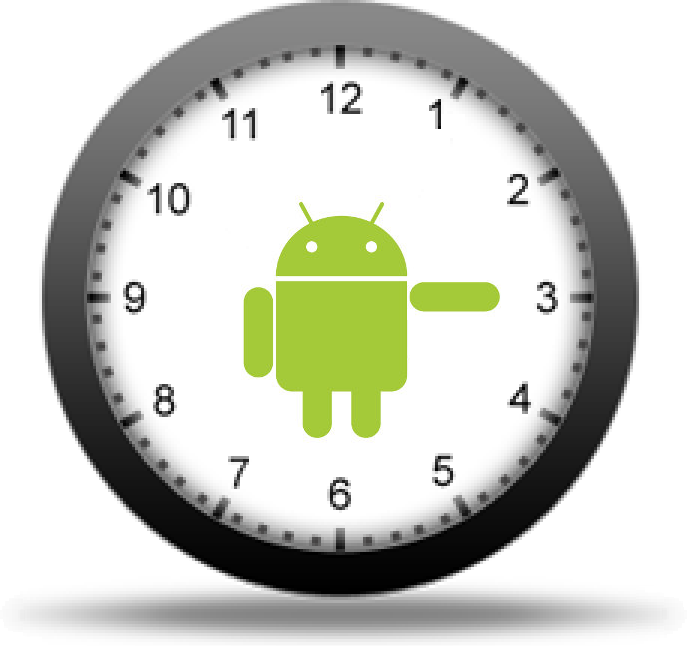
\includegraphics[scale=0.575]{Images/frontpage_pic.png}
\end{center}
\end{figure}

\end{comment}
\newpage
\thispagestyle{empty}
\mbox{}
\input{Chapters/titelblad.tex}
\newpage
\newpage
\thispagestyle{empty}
\mbox{}
\tableofcontents
\newpage
\thispagestyle{empty}
\mbox{}
\chapter{Introduction}
\input{Chapters/Res.tex} %done.p1 
\section{Real-time systems}
\input{Chapters/realTime.tex} % done.p1
\section{Motivation}
In order to describe the context of the system, we -- as a multi project group -- will in the following state the motivation of the project, the group of people we are aiming at helping, the technological platform chosen, the used development method, followed by a problem definition, a system description and architecture, and the conducted usability test.

\section{Motivation}
As this is a student report written as part of a learning project, we are required to comply with the study regulation.
The main areas of focus, according to the study regulation, are: multi project management and quality assurance in the form of requirements analysis, requirements management, and testing.
The goal is to create a comprehensive software system, across multiple project groups, in order to enhance our competences in analysis, design, implementation, and evaluation of software applications in regards to the system requirements\cite{studyreg}.

This project builds on top of a previous project, and is further developed, with the aim of having other students continue the development.
The goal of the project, we are building on top of, is to create a touch based tablet system to support children and their guardians in everyday scenarios.%done.p1
\section{Problem statement} 
\input{Chapters/problemstatement.tex}%done.p1


\chapter{Theory of RTS}
\label{chap:rts}
\section{Hard and soft real-time}
\input{Chapters/HardAndSoft.tex}%done.p1
\section{Reliability}
\input{Chapters/fault.tex}%done.p1
\section{Tasks}
\input{Chapters/tasktheory.tex}%done.p1
\section{Scheduling}
\input{Chapters/schedulingTheory.tex}%done.p1


\chapter{Analysis}
\label{AnalChap}
\input{Chapters/AnalIntro.tex}%done.p1
%\section{RTS aspects}
%\input{Chapters/RTSaspects.tex}
\section{LEGO NXT 2.0}
\input{Chapters/NXT.tex} %done.p1

\section{Programming language}
\label{leJosStuff}
\input{Chapters/programminglanguages.tex}%done.p1

\section{Sensors}
\label{secSen}
\input{Chapters/senIntro.tex}%done.p1
\subsection{Color Sensor}
\label{secColorSensor}
\input{Chapters/ColorSensor.tex}%done.p1
\subsection{Compass}
\label{secCompassSensor}
\input{Chapters/compass.tex}%done.p1
\subsection{NXTSumoEyes}
\label{secsumoSensor}
\input{Chapters/sumoExp.tex}%done.p1
\subsection{Ultrasonic Sensor}
\label{section:usexp}
\input{Chapters/usexp.tex}%done.p1
\subsection{Touch Sensor}
\input{Chapters/touchsensor.tex}%done.p1
\section{Actuators}
\label{secAct}
\input{Chapters/Actuatorintro.tex}%done.p1
\subsection{Interactive Servo Motor}
\label{secDaMotors}
\input{Chapters/ServoMotor.tex}%done.p1

\begin{comment} Skal måske bruges hvis det mangler når vi læser igennem senere.
\subsection{Fire and hit system}
\input{Chapters/shootingsystem.tex}
\end{comment}

\chapter{Design}
\label{DesignSec}
\input{Chapters/Designgrid.tex}%done.p1
\section{Vehicle}
\label{vehicledesign}
\input{Chapters/Designvehicle.tex}%done.p1
\section{Tower}
\label{towerdesign}
\input{Chapters/Designtower.tex}%done.p1
\section{Real-time aspects}
\input{Chapters/RealTimeAspects.tex}%done.p1
\section{Tasks}
\label{sect:dtasks}
\input{Chapters/tasksv2.tex}%done.p1
%section RTA, is in the file.
\input{Chapters/RTA.tex}%done.p1






\chapter{Implementation}
\label{chap:impl}
\input{Chapters/impl.tex}%done.p1
\section{Vehicle}
\input{Chapters/implVehicle.tex}%done.p1
\section{Tower}
\input{Chapters/ImplTower.tex}%done.p1





\chapter{Conclusion}
\chapter{Conclusion}

\textit{In this chapter, we will present the conclusion of the project.}\newline
\\
The problem definition states:
\begin{quote}
How can we ease the daily life for children with ASD and their guardians, while complying with the study regulation?
\end{quote}
\\
We have designed a product that should help ease the use of pictograms. 
PARROT should help organize and ease access and use of pictograms. This allows for many of these to be handled simultaneously, without the need of the many physical pictograms and their bulky folders as mentioned in the analysis.\newline
It also gives the functionality to play sound, which could help some of the children learn the spoken language while using the pictograms to communicate. 
The idea of handling pictograms digitally also opens opportunities otherwise not easily accessible for the guardians.
For instance, we can change PARROT's colors according to the needs of the individual child. This include the colors for the different categories as well as those of the speech board.
The guardian can modify the categories and organize them according to the needs of the child.\newline
Since we have developed an application based on the needs of a third party, have been part of a multi project, and have performed dynamic blackbox testing as well as whitebox usability testing, we have upheld the goals of the study regulation.\newline

The whole project have been part of a greater multi project with five groups participating. 
As such we have not made a individual product, but one that is part of a greater product, GIRAF.  
GIRAF is not yet finished, but is hopefully going to be continued by other students on future semesters, so that it can become a product worthy of being used in the aforementioned institutions.\newline
As part of the multi project we have been using an agile development method, SCRUM.
Using SCRUM we have not spent the start of the semester analyzing the whole system, and designing it from the start. Instead we have analyzed and designed parts of the system one sprint at the time.
In previous semesters, we have wasted time on analyzing functionality that was never written, which was not the case in this semester.\newline
\\
\textit{This chapter presented the conclusion.}
\chapter{Future work}
\input{Chapters/Furtherwork.tex}

\appendix
\chapter{Routes for color sensor test}
\label{colorTestAppendix}
\input{Chapters/AppColorTest.tex}
\chapter{Code for color Sensor test}
\label{appColorTestCode}
\input{Chapters/appColorTestCode.tex}
\chapter{Code for Compass Sensor test}
\label{appCompasTestCode}
\input{Chapters/appCompasTestCode.tex}
\chapter{Code for motor test}
\label{appMotorTestCode}
\input{Chapters/appMotorTestCode.tex}
\chapter{Ultrasonic tests}
\input{Chapters/appultasonic.tex}
\chapter{Code for platform test}
\label{platformtest}
\input{Chapters/platformtestcode.tex}

\bibliographystyle{plain}
\bibliography{bib/bib}

\listoffigures
\listoftables
\lstlistoflistings

\end{document}
